\begin{figure*}[htbp]
  \noindent\makebox[1.1\textwidth]{
  \begin{subfigure}[b]{0.7\textwidth}
      \centering
      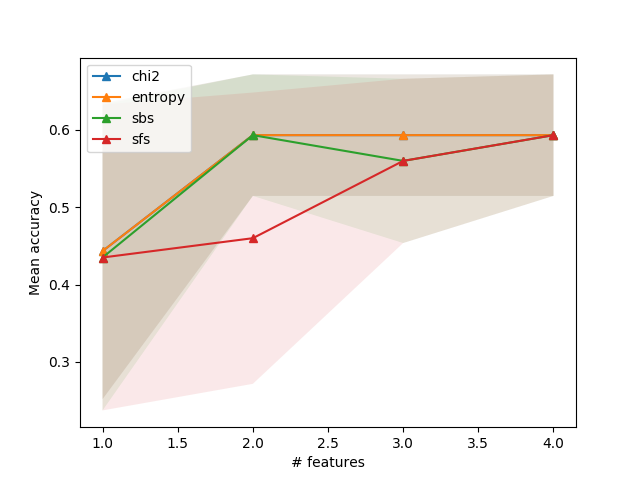
\includegraphics[width=\textwidth]{../plots_with_std_fill/SVMd1.png}
      \caption[]%
      {{\small}}
      \label{fig:SVM_MIAS}
  \end{subfigure}
  \hfill
  \begin{subfigure}[b]{0.7\textwidth}
      \centering
      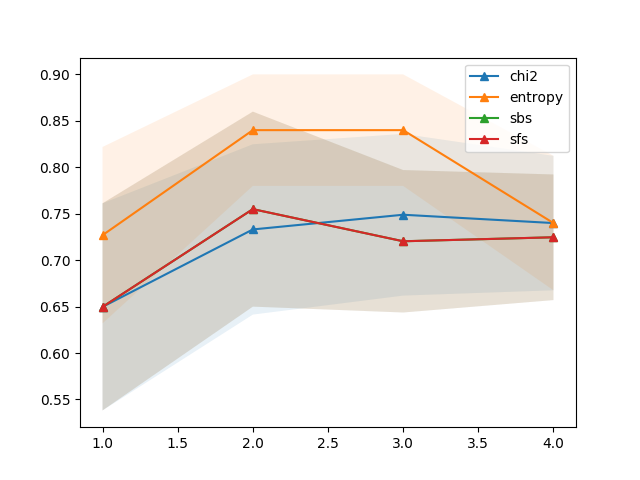
\includegraphics[width=\textwidth]{../plots_with_std_fill/SVMd2.png}
      \caption[]%
      {{\small}}
      \label{fig:SVM_EN}
  \end{subfigure}
  }
  \vskip
  \baselineskip
  \noindent\makebox[1.1\textwidth]{
  \begin{subfigure}[b]{0.7\textwidth}
      \centering
      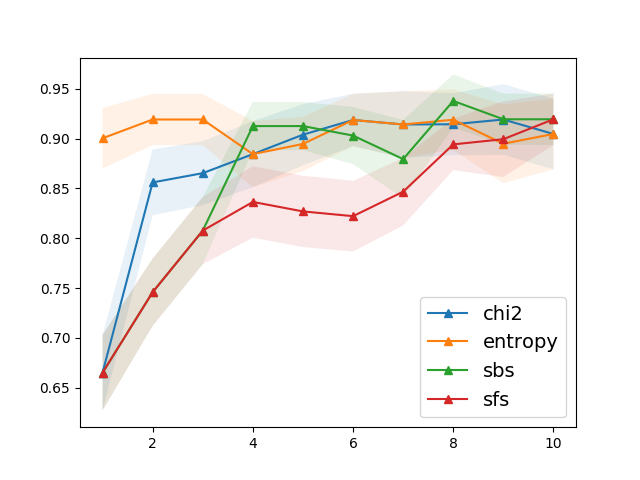
\includegraphics[width=\textwidth]{../plots_with_std_fill/SVMd3.png}
      \caption[]%
      {{\small}}
      \label{fig:SVM_RHH}
  \end{subfigure}
  \quad
  \begin{subfigure}[b]{0.7\textwidth}
      \centering
      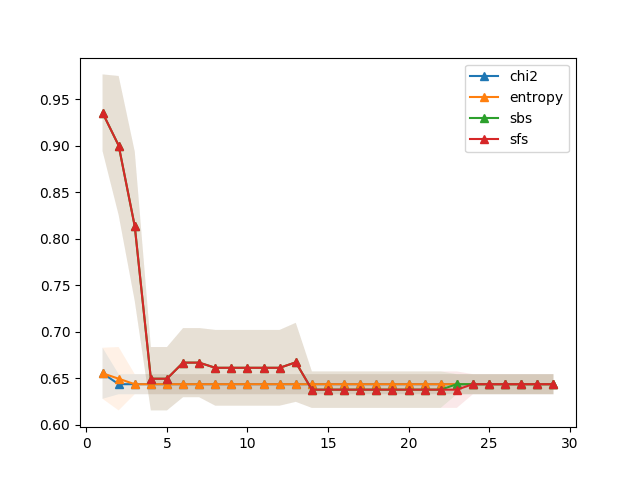
\includegraphics[width=\textwidth]{../plots_with_std_fill/SVMd4.png}
      \caption[]%
      {{\small}}
      \label{fig:SVM_WBCD}
  \end{subfigure}
  }
  \caption[]
  {\small
    Classifier SVM. Each plot corresponds to datasets (a) MIAS, (b) EN, (c) RHH and (d) WBCD. x-axis is number of features, y-axis is mean accuracy achieved by corresponding feature selection method. Shaded area represent the standard error for each FS-method.
  }
  \label{fig:plots_SVM}
\end{figure*}
